\chapter{Hyperkinetic movement disorder analysis}
\label{ch:nemo}

\textit{
In this chapter, we present a real-world application for the dynamic projection methods introduced in \cref{ch:proj-eval,ch:proj-algo}. The context of our application is the analysis of hyperkinetic movement disorders. These disorders manifest as abnormal involuntary movements that highly affect the quality of life of the people who suffer from them. These involuntary movements may present a wide range of tendencies: they may be regular and rhythmic (tremors); swift ``lightning-like'' jerks or twitches (myoclonus); or sustained and repetitive movements resulting in abnormal postures (dystonia); they may present a random, brief, and non-rhythmic character (chorea); or can be temporarily suppressible jerks (tics). The diagnosis of these disorders is carried out via careful professional observation. It can be extra challenging due to the circumstantial emergence of certain behaviors (triggered by specific postures or tasks) and their manifestation via compound movements, including a combination of the various hyperkinesias. All these factors lead to professionals often disagreeing with diagnosis. 
This chapter focuses on electromyography (EMG) and motion sensors (accelerometry) data collected from patients with hyperkinetic movement disorders while performing motor tasks. We show how we transform these data and study them with a visual analytics tool based on dynamic projections. We discuss an example of data exploration that leads to valuable clinical insights.
}

\vspace{5mm} %5mm vertical space


% \noindent \textbf{Abstract:}

\section{Introduction}


Hyperkinetic movement disorders are a class of disorders that are characterized by excessive and involuntary motor movements. These disorders include a range of different phenotypes\footnote{A phenotype is any observable characteristic or trait of a disease, such as morphology, development, biochemical or physiological properties, or behavior, without any implication of mechanism.} such as myoclonus, dystonia, tremor, chorea and tics. Since the clinical presentation and etiology differs among these disorders, each of these disorders requires a different clinical strategy. These strategies differ in e.g., the choice of additional diagnostic tests, medication prescriptions, and deep brain stimulation targets. For the correct strategy, it is of utmost importance to ensure accurate phenotypic classification. As most hyperkinetic movement disorders have no clear anatomical brain abnormalities, classification is based on clinical definitions and thus on expert opinion. What makes this increasingly difficult is that complex and mixed forms of phenotypes occur in many patients, and many clinical features of these hyperkinetic movement disorders also correspond to clinical features of other disorders classes such as ataxia, spasticity, and functional movement disorders. Moreover, there is large inter- and intra-observer classification variability in expert clinicians \citep{VANDERVEEN2021176,defazio,eggink,beghi,vandersalm}.

To improve hyperkinetic movement disorder phenotyping, the Next Move in Movement Disorders (NEMO) \citep{NEMO} study was set up at the University Medical Center Groningen, The Netherlands. The aim of this study is to build computer-aided hyperkinetic movement disorder classification tools to assist healthcare professionals in phenotyping (see further Sec.~\ref{experiment}). 

The current chapter focuses on the EMG and accelerometry data of the NEMO study. EMG is a technique that measures electrical activity in skeletal muscles. This can either be done by placing an electrode inside the muscle of interest, or on the skin above the muscle. The latter technique is referred to as surface EMG and is employed in the current study. The simplest application of EMG is to determine whether a muscle is active. Accelerometry data collects information on the 3D motion of several sensors placed on the body of a subject that performs a task.

The above EMG and accelerometry data contains a wealth of information describing the dynamics of a subject that performs a task involving motion. The underlying assumption we have, on which the NEMO study is also based, is that analyzing such data will allow us to find patterns specific to particular types of hyperkinetic movement disorders. In turn, this will help the design of computer-aided systems for disorder characterization and classification.

However, the joint EMG and acceletrometry data is large (in terms of the number of sample points), high-dimensional (has many independent variables), and temporal -- and, as such, it is challenging to analyze and interpret. On the other hand, this is precisely the type of data for which our dynamic projection methods presented in the previous chapters were designed.

We explore the idea of using dimensionality reduction (DR) methods on the EMG and accelerometry data in order to support the exploration of the data collected in the NEMO experiments. We are not directly trying to solve the clinical problem of phenotypical classification of movement disorders. This is a much harder problem, the pursuit of which would encompass one thesis of its own. Our goal is to understand the technical challenges associated with applying DR methods to such complex time-dependent EMG and accelerometry data sets to support effective data exploration. We show evidence that the dynamic projection methods we proposed in earlier chapters are suitable to handle such complex data and generate interesting insights in this particular clinical setting, opening new possible paths of analysis, which were previously unavailable due to technical limitations. 


\section{Related work}
\label{sec:nemo_related}
%
In clinical practice, EMG is often combined with accelerometry, a method that measures the acceleration of limb displacement rather than muscle activity. Measurements are typically performed during rest or during diagnostic movement tasks and clinically assessed using several characteristics of the patient’s movement pattern, such as muscle activation patterns, movement burst duration, and frequency analysis \citep{VANDERVEEN2021176}.

More advanced analyses to help support the classification of tremor, myoclonus, or dystonia focus on the electrophysiological autospectrum to investigate the frequency distribution using Fourier transforms, standard coherence analysis to investigate the dependence of multiple signals in the frequency domain, wavelet coherence analysis to investigate the variation of coherence in the time domain, cumulant density to investigate the relationship between signals in the time domain, and Jerk-locked back-averaging to investigate signal relationships during events of interest (\emph{i.e.}, jerks) across measurement modalities, respectively~\citep{nijmeijer2014emg, tijssen2000frequency, grosse2004patterns, kramer2018wavelet, Stouwe2015, grosse2003abnormal}.

Unfortunately, there are several known limitations to the diagnostic value of EMG and accelerometry features in hyperkinetic movement disorder phenotyping, three of which we will discuss briefly. First, high-level evidence for the differentiating value of each feature is sparse. Only a limited number of diagnostic test accuracy studies exist, most of which report on tremor patients. Many of the features that are currently a part of the diagnostic criteria for movement disorders have only been reported in descriptive studies, and have not been compared between patient groups, \emph{e.g.}, in myoclonus versus tremor patients. Hence, incorporating these features in clinical practice is largely based on clinical observations and expert opinion. Secondly, proper application of EMG and accelerometry techniques and interpretation of the results requires training and experience. Both practice and quality range widely between medical centers, and diagnostic accuracy are highest in specialized centers. Thirdly, the application of EMG and accelerometry features is complicated by the inherent nature of movement disorders themselves: As all of these disorders are defined by excessive involuntary movement, it is only to be expected that many movement disorder phenotypes share overlapping features. Combined, these three factors currently limit the diagnostic value of EMG and accelerometry features for movement disorders.

\section{Hyperkinectic movement disorders and experiment design} \label{experiment}
%
%
The experimental design of the NEMO study is described in detail in \citep{NEMO}. In short, a large data set is being collected from hyperkinetic movement disorder patients (20 dystonia, 20 myoclonus, and 20 tremor patients) and 40 healthy controls. In the future, the study aims to include additional patient groups. Importantly, disorder phenotype classification in this data set is based on independent expert panel agreement.

In the study, participants perform 36 motor tasks during a movement registration setting, and 1 motor and 3 non-motor tasks in neuroimaging settings. During movement registration, data is collected using electromyography (EMG), motion sensors (accelerometry), and 2D and 3D video. In the neuroimaging settings, data is measured using positron emission tomography (PET) and functional magnetic resonance imaging (fMRI).  

Participants are only eligible for inclusion if they are at least 16 years old and healthy participants cannot be first-degree relatives of patients with hyperkinetic movement disorders. 

The current chapter focuses on the data from the movement registration. During this setting, participants performed 36 tasks that are used in the clinical setting. Tasks were selected based on panel discussions with seven movement disorders, neuropediatric, and neurorehabilitation specialists with extensive experience in the fields of dystonia, myoclonus, tremor, chorea, tics, ataxia or spasticity to ensure coverage of all disorders.


\section{Visual analysis of collected data}
\label{sec:nemo_va}
%
Our goal was to design a visual analytics tool that supports exploring the motion data generated in the NEMO project. This is important given that the data is vast and has many axes that can be explored.
% : There are over 100 patients, over 30 tasks, and 16 motion units which record accelerometer (3 axes), gyroscope (3 axes), and EMG (1 dimension) at up to 4370 samples per second, plus 2D and 3D video, and, for some experiments, additional modalities, such as page scans. 
Exploring this large data corpus is challenging. Thus, we aim to provide medical professionals with a tool to \emph{navigate} through and generate valuable \emph{insights} from patient motion patterns effectively and efficiently. Our tool aims to support a wide range of capabilities, such as identifying clusters, outliers, erratic observations, or failures in the data collection. It also aims to support medical analysis tasks, such as comparing various hyperkinesias to healthy behavior or identifying under which circumstances certain abnormal tendencies become incident. In both cases, we must be able to compare the severity and variability of their manifestation.

Another essential aspect our tool aims to provide is \emph{meta-analysis}, where we want to know which combinations of sensors, tasks, patient groups, and preprocessing transformations generate representative data that may be useful in further investigation steps. Such meta-analysis is helpful if we want to build a classifier and keep only ``good data'' (\emph{i.e.}, which discriminates between the classes we aim to infer) or if we want to understand the minimal resources (sensors and/or tasks) needed when performing data collection in a third-party, more resource-constrained, clinic.

We envisioned a visual analytics design that supports Shneiderman's mantra: Overview first, zoom and filter, then details-on-demand. Nevertheless, to generate interactive visualizations that implement these, we need to perform a series of transformations on the raw data. These are explained in detail next (see also \cref{fig:nemo-pipe} for an overview of the tool's pipeline).

\begin{figure*}[ht]
\centering
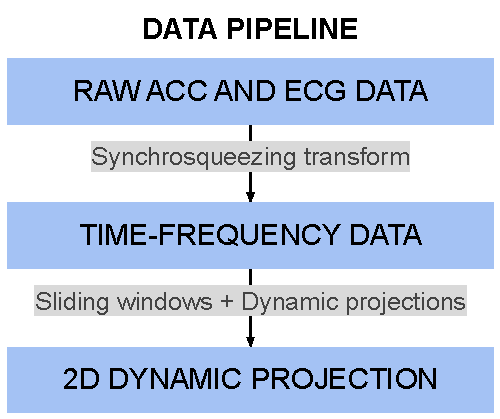
\includegraphics[width=.5\linewidth]{figures/nemo/simple-pipeline.pdf}
\caption{Data transformation pipeline.}
\label{fig:nemo-pipe}
\end{figure*}

\subsection{Raw data visual inspection}
\label{sec:nemo_pipeline_rawdata}
%
To illustrate all the data transformations, we begin by inspecting the raw data given by an accelerometer sensor placed on the subject's right hand. The task we will investigate is described as ``Arms stretched forward, wrists straight, palms down, and suppress involuntary movements'' (\cref{fig:hands}).

\begin{figure*}[ht]
\centering
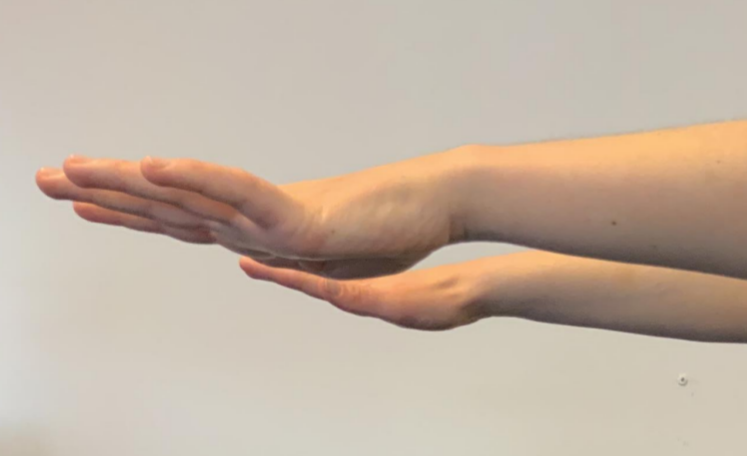
\includegraphics[width=.5\linewidth]{figures/nemo/hands.png}
\caption{Static position with arms and hands stretched out in front of body for 20-30 seconds. The subject tries to suppress any involuntary movements.}
\label{fig:hands}
\end{figure*}

\cref{fig:acc} shows the accelerometer data collected during the experiments for three subjects. For each subject, we see three colored curves corresponding to the X (red), Y (green), and Z (blue) axes measurements of a sensor placed on the right opisthenar (back of the right hand). The recording rate is 148 samples per second. The curves are offset from each other because the sensor reads the subject's movement acceleration as well as the Earth's gravity. An accelerometer at rest on the surface of the Earth will measure an upwards acceleration due to the gravity of $g \approx 9.81 m/s^2$. 

The same sensor unit also records gyroscopic and EMG data. We decided to ignore EMG data due to the additional complexity introduced in the non-standard preprocessing steps that (usually) involve noise rejection/filtering, whitening, gain scaling, demodulation, smoothing, and relinearization. For the  discussion next, we will only focus on accelerometer data.

The three subplots in \cref{fig:acc} show data acceleration corresponding to three subjects: 
\begin{itemize}
  \item Patient \textit{a} (top panel) is the \emph{healthy} control: The curves are very close to straight lines. The small oscillations indicate very low-magnitude movement since it is impossible, even for a healthy person, to hold this position perfectly still.
  \item Patient \textit{b} (middle panel) measurements show a very rhythmic and regular \emph{tremor} of average magnitude. This patient was actually diagnosed with essential tremor, the most common trembling disorder, often confused with Parkinson's disease.
  \item Patient \textit{c} (bottom panel) shows curves with high amplitude random non-rhythmic movements. This patient was actually diagnosed with \emph{chorea}. 
  %ALEX: the following isn't relevant for the thesis chapter 
  % \eduardo{Are we allowed to upload censored videos to a website?}
\end{itemize}
 

\begin{figure*}[ht]
\centering
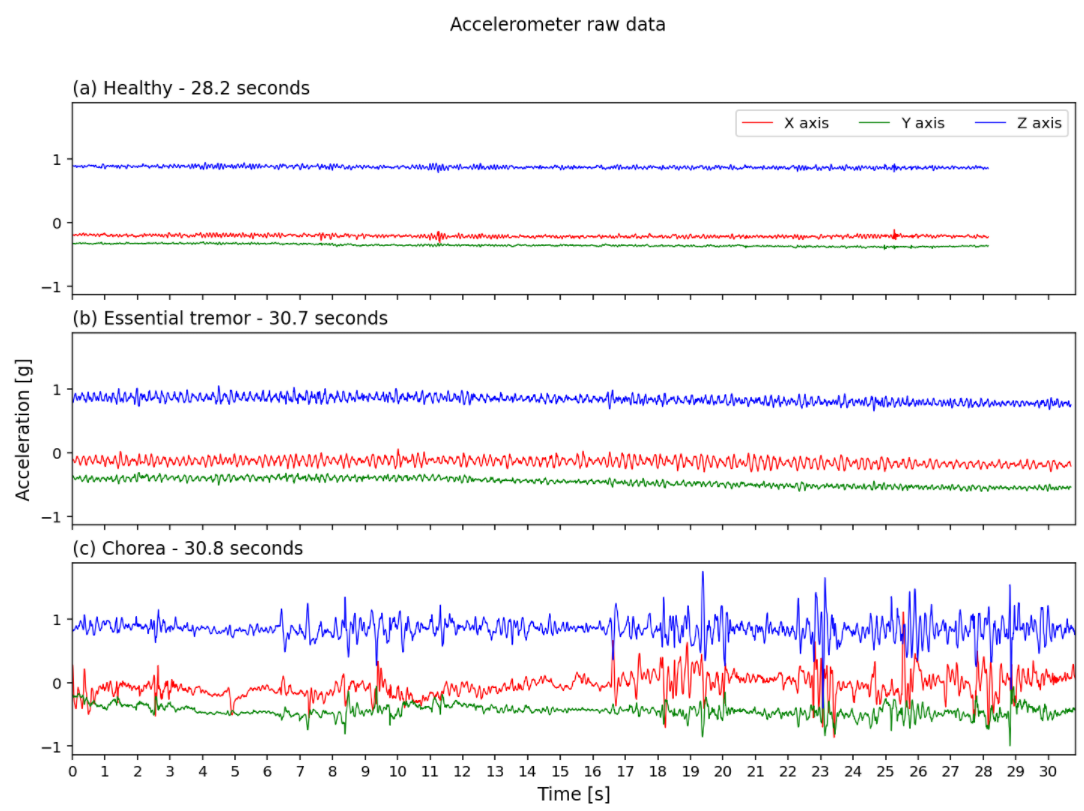
\includegraphics[width=\linewidth]{figures/nemo/acc2.png}
\caption{Accelerometer data for three subjects classified by experts as (a) healthy, (b) diagnosed with essential tremor, and (c) diagnosed with chorea. The data corresponds to a task where the subject must hold their hands as still as possible in the position suggested in Fig. \ref{fig:hands}.
Each subplot corresponds to the accelerometer data collected during the experiment and is broken down into three orthogonal components (X, Y, and Z-axis). 
%ALEX: not relevant for the thesis chapter
% \eduardo{Are we allowed to upload censored videos to a website?}
}
\label{fig:acc}
\end{figure*}

\subsection{Time-frequency data analysis}
%
The simple graphs in \cref{fig:acc} are handy for reasoning about the disorders and understanding their behavior over time. However, they do not tell the whole story. We can get a different perspective on the data that reveals relevant information hidden in the raw signal by decomposing it into the frequencies that form it. This can be done in two ways, \emph{i.e.}, using a frequency-domain representation or alternatively a time-frequency representation. The former assumes that the signal is stationary. Given the nature of our experiments, we know that our data does not fall in this category. Hence, we do not consider frequency-domain representations such as the Fourier Transform. In contrast, a time-frequency representation allows us to reason about how the frequency-domain (the spectrum) of a signal changes \emph{over time}. We explore this representation next.

The technique we use for time-frequency analysis is called Synchrosqueezing Wavelet Transform (SWT)~ \citep{MIHALEC2016324}. It is an improvement over the original Wavelet transform \citep{wavelet} which provides a sparser, sharper, noise-robust, and partly denoised representation of the time-frequency information. Figure~\ref{fig:freq}, also called a spectrogram, shows a visual representation of the SWT for the data shown earlier in Fig.~\ref{fig:acc}. The horizontal axis indicates, again, time. For every time moment, the vertical axis plots a frequency spectrum for that moment, where the magnitude (presence) of a certain frequency is color-coded (black is low, white is high, magnitude).
%ALEX: this is pretty enough info for this context
%\eduardo{how deep do we want to go here?}

This time-frequency representation can be of great relevance for the diagnosis of motion disorders. For example, studies suggest that 95\% of essential tremor cases exhibited frequencies in the 5--8Hz range. If we examine \cref{fig:freq}(b), we can see that,  through the whole experiment, there is a defined presence of frequencies in this precise range, showing a common and insuppressible tendency to the involuntary movement. We do not see the same ``horizontal line'' in that frequency range for patients \textit{a} and \textit{c}. Patient \textit{a} can hold his/her hand in a much more stable position, which translates into a darker spectrogram (less energy). In contrast, patient \textit{c} performs high amplitude random non-rhythmic movements characteristic of chorea. The light colors in the spectrogram represent the high amplitude, and the ``random non-rhythmic'' aspect can be read as having no constant lines in the time-frequency representation, as seen on patient \textit{b}. Having both representations (\cref{fig:acc,fig:freq}) side-by-side helps us understand the phenomena as a whole. 
% https://www.ncbi.nlm.nih.gov/pmc/articles/PMC3475963/

For our purposes, the time-frequency representation is essential as it facilitates comparison between signals. Methods for computing similarity of signals in the time-domain (raw signals) exist, \emph{e.g.}, RMSE, cross-correlation, and Dynamic Time Warping~\citep{Gupta1996}). However, these can be significantly affected by the phase shift and minor differences in frequency. By making comparisons in the time-frequency domain, we get a better, more reliable representation that is better suited for the next steps of our pipeline.

%The sensor reads acceleration in three orthogonal axes (X, Y, Z). For the next figures, we will focus on the Z axis, which points up/down for the hands shown in \cref{fig:hands}.

\begin{figure*}[ht]
\centering
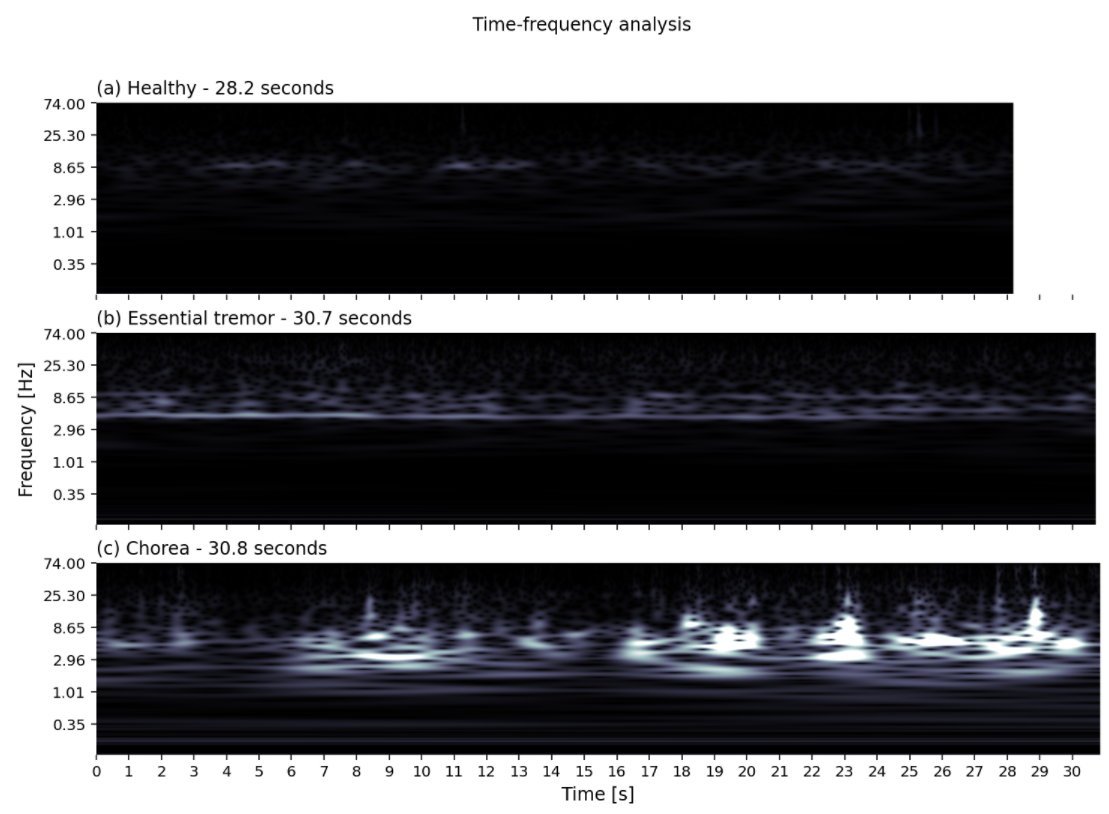
\includegraphics[width=\linewidth]{figures/nemo/freq2.png}
\caption{Time-frequency representation of the acceleration of the Z axis (blue) in Fig. \ref{fig:acc}. This is the vertical axis which points up/down for the hands shown in \cref{fig:hands}. Light colors represent high energy in the spectral distribution, \emph{i.e.}, there is a large amplitude component in the subject's movement associated to a particular frequency or frequency distribution. 
%ALEX: not needed, it is actually explained in the text.
%\eduardo{add colormap}
}
\label{fig:freq}
\end{figure*}

\subsection{Data normalization}
\label{sec:nemo_pipeline_datanorm}
%
The acceleration time plots and spectrograms discussed so far are quite effective in studying the data of a \emph{single} subject. However, as outlined earlier in the chapter, our goal is to compare \emph{multiple} subjects in order to find out which data aspects make them similar or different. For this, we need a way to `normalize' the collected data collected from each measurement (experiment) so that it becomes comparable across multiple measurements.

As seen in \cref{fig:freq}, time-frequency information can vary slightly from recording to recording. These recordings can have different lengths and different frequency ranges. Both of these are due to the difference in experiment duration. Experiments that last more have longer spectrograms and a higher frequency range since we can detect more frequencies in the lower range. The sampling rate of the sensor sets the upper range of the frequency spectrum. The accelerometers we used can collect 148 readings per second, so the maximum frequency we can detect is 74 Hz. We also limit our frequency range to 100 logarithmic bins in the range of $0-74$ Hz. 

To get our data in a uniform and easily comparable format, we use the Sliding Window method as illustrated in \cref{fig:sliding}. In this example, we set a stride $t_s$ of 1 second and a time-window width $t_w$ of 5 seconds. Each such time window will thus aggregate the data falling within it into a single (high-dimensional) measurement. Increasing $t_w$ introduces more filtering, which can be desirable when the data is highly noisy (or we are interested mainly in lower frequencies). Increasing $t_s$ decreases the total number of sample points (along the time axis) that we reduce our data to.
We can change the parameters $t_s$ and $t_w$ on the fly to generate visualizations of different ``resolutions'', as discussed next.

\begin{figure*}[ht]
\centering
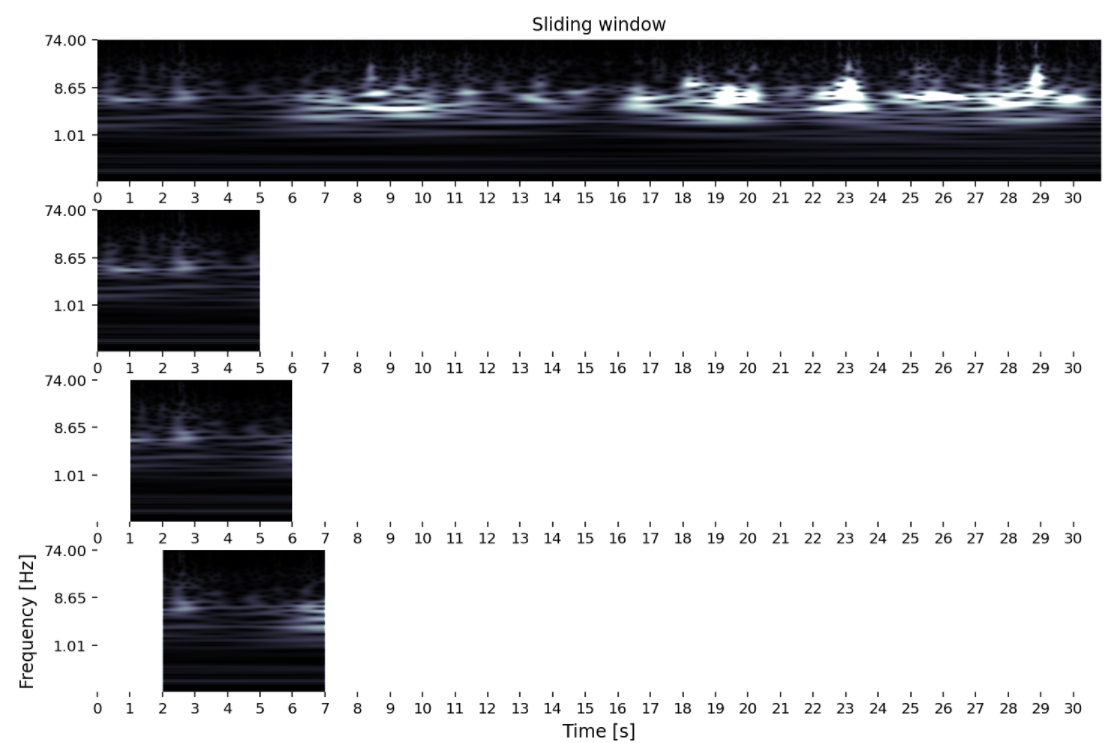
\includegraphics[width=\linewidth]{figures/nemo/sliding.png}
\caption{Before we project our data, we subdivide each spectrogram using the Sliding Window method. In this example, we use a window width of $t_w=5$ seconds and a stride of $t_s=1$ second to partition the data from Fig.~\ref{fig:freq}c.}
\label{fig:sliding}
\end{figure*}

\subsection{Visualizing the data with dynamic projections}
\label{sec:nemo_pipeline_dr}
%
Since our data is multidimensional and temporal, we use dynamic projections to obtain further insights into our dataset.
For this tool, we implemented three of the dynamic projection methods introduced in the previous two chapters. These are G-PCA, G-tSNE (\cref{ch:proj-eval}), and PCD-tSNE (\cref{ch:proj-algo}). 
As discussed earlier in the thesis, G-PCA and PCD-tSNE are methods that balance visual quality and temporal stability, but they each have pros and cons. PCD-tSNE has better neighborhood and distance preservation than G-PCA and comparable stability. Its main drawback for this particular application is that a few parameters need to be adjusted, which adds an undesired level of uncertainty when interactively exploring the data. This same trait outside of an interactive setting can be advantageous, as it allows us to create projections that borrow characteristics from both PCA and tSNE-based methods, as previously discussed in \cref{sec:results}. % chapter 6
G-tSNE is a relatively unstable technique, as benchmarked in \cref{ch:proj-eval}. However, it still provides interesting (non-temporal) insights into the high-dimensional structure of the data.

\cref{fig:nemo1-projections} shows the data from patients \textit{a}, \textit{b}, and \textit{c} projected using the three DR methods mention above. In each projection, we see three curves (trails). Each curve describes the behavior over time of one patient -- simply put, the patient can be seen as `moving along the curve' in projection space. As the spectral signatures of the different patients are different from each other, we see that the trails do not overlap. We also observe how PCD-tSNE creates a projection that borrows traits from both G-PCA and G-tSNE. The general position of all clusters and shape of the (c) trail resemble that of G-PCA, while the focus on intercluster neighborhood preservation for trails (a) and (b) (materialized as expanded clusters) are traits derived from the t-SNE influence.

\begin{figure*}[ht]
\centering
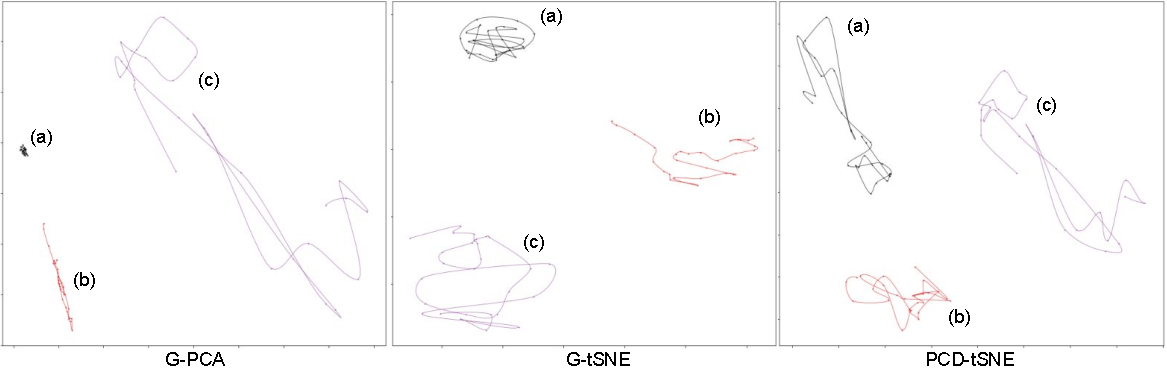
\includegraphics[width=\linewidth]{figures/nemo/nemo1-projections.pdf}
\caption{The last step of the pipeline is to project (using dynamic methods) the data that has been subdivided by the Sliding Window method. Our tool supports 3 dynamic projection methods: G-PCA, PCD-tSNE, and G-tSNE. We visualize the dynamic projections as trails, where we connect the consecutive spectrum ``windows'' via Akima spline \citep{akima}. The data corresponds to the patients presented in \cref{fig:acc,fig:freq}.}
\label{fig:nemo1-projections}
\end{figure*}

\section{Data exploration}
\label{sec:nemo_data_exploration}
%
This section presents an example of the type of data exploration that our visual analytics tool supports. 

% The NEMO project has over 150 participants diagnosed with six different disorders. Each participant performed 36 tasks whiled being measured by tens of sensors.
% Jelle this is already covered in \ref{experiment}

There are many ways to conduct data exploration, depending on the goal of the analysis. Some relevant examples from a clinical standpoint are
\begin{itemize}
  \item understand the behavior of different patients or patient groups for a given task; 
  \item given new patient measurements, find patients with similar movement characteristics to assist diagnosis;
  \item explore the movements that led to a specific diagnosis;
  \item study the erratic/circumstantial nature of the appearance of certain symptoms;
  \item understand how different tasks induce different behaviors on specific patients or patient groups. 
\end{itemize}

In the following, we will describe an example analysis that will focus on the first goal. We want to understand the behavior of essential tremor patients \emph{vs} healthy controls in the context of the task described as ``arms stretched forward, wrists straight, palms down, and suppress involuntary movements'' (\cref{fig:hands}). In total, we have 24 healthy subjects and 11 tremor patients. For the next figures, we will select to use the reading from the Z-axis of the accelerometer sensor placed on the subject's right hand. 

Once we select the data subset of interest, we need to choose how to project the data. \cref{fig:exp1-gpca} displays two G-PCA projections. The only difference is the size of the sliding window $t_w$ (\cref{fig:sliding}), which translates into the resolution and smoothness of the projection. The left projection has a sliding window size of $t_w=1$ second and a stride of $t_s=1$ second, meaning that there is no overlap between the consecutive windows, leading to more jagged trails. The right projection has a window size of $t_w=5$ seconds instead, so consecutive windows share part of the same data, leading to a longer representation of temporal phenomena and smoother trails. The choice of window size and window stride also depends on the amount of data we are projecting, \emph{i.e.}, number of patients and length of experiments. We will use an empirically found window size of $t_w=5$ seconds and a stride of $t_s=1$ second for the following figures. 

\begin{figure}
\centering
\begin{minipage}{.5\textwidth}
  \centering
  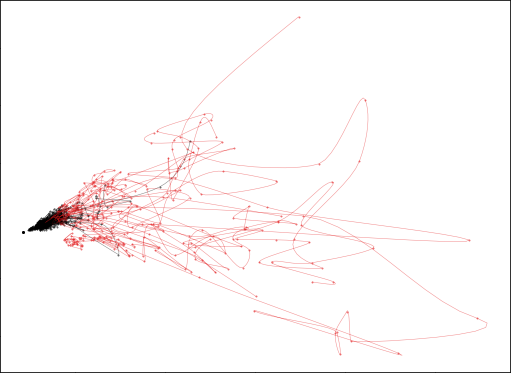
\includegraphics[width=\linewidth]{figures/nemo/exp1.png}
  % \captionof{figure}{A figure}
  % \label{fig:exp1-gpca-1s-1s}
\end{minipage}%
\begin{minipage}{.5\textwidth}
  \centering
  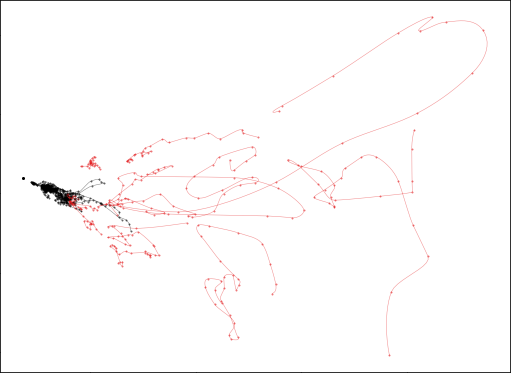
\includegraphics[width=\linewidth]{figures/nemo/exp1-5s-window.png}
  % \captionof{figure}{Another figure}
  % \label{fig:exp1-gpca-5s-1s}
\end{minipage}
\caption{G-PCA projection of 24 healthy (black) and 11 tremor (red) patients with window width and stride of [1s, 1s] on the left and [5s, 1s] on the right.}
\label{fig:exp1-gpca}
\end{figure}


With the projected data in front of us, we can start making some observations. We see that most healthy patients (black trails) cluster together in a tight formation in the ``center'' of the projection, while the tremor patients' trails tend to be located to the right of this cluster and have a broader spread. The angle and distance from the central cluster must portray some traits in the data, but we cannot confirm anything just yet.   

To better understand the overall structure of the projection, we  start by looking at a couple of trails drawn in its periphery. We start selecting patient 91 (\cref{fig:exp1-9196}-left). Our tool also displays the video recording of the experiment (not shown here due to privacy concerns). 

Patient 91 presents a unique behavior. Looking at the raw signal and spectrogram, we can tell that in the initial 2-3 seconds, there is a presence of medium amplitude tremors, followed by high amplitude tremors until second 13, and then a significant reduction in the intensity until the end of the experiment. We also see that the movement is decomposed into a ``sharp'' spectrum, mainly focused on around 5 Hz. One hypothesis is that the patient can suppress involuntary movements after considerable effort, which is only possible after a few seconds into the experiment. This dynamic translates in a particular projection trail (top-left): The trail starts a certain distance away from the center of the projection, characteristic of ``unhealthy'' behavior, and then ``shoots'' away to the top left as tremor intensity increases, only to finally move closer to the center of the projection, close to the healthy cluster as the amplitude is reduced. This hints that the distance from the ``center'' of the projection is related to the energy in the signal, that is, how large the movements are. 

The three plots on the right portray the data collected from patient 96 (\cref{fig:exp1-9196}-right). This patient was also diagnosed with important tremors, but its manifestation shows essential differences compared to patient 91. Patient 96 shows a more constant tremor. The amplitude is constantly high, showing that the patient cannot suppress the movement. Another dissimilarity comes in the signature of the tremor: Patient 91 has a ``sharp'' histogram, meaning that his tremor has very sinusoidal tendencies, while the same is not valid for patient 96, given the presence of high energy high frequencies on the spectrum. Upon detailed inspection of the video recording, this can be related to the fact that patient 96's tremor has a more lateral tendency (side-to-side instead of up-and-down). We also notice extra movement at the beginning of the recording as the patient gets into position, which can be identified in the projection as abnormal movements that make the trails start at the right-bottom at a considerable distance from where the rest of the trail is located.  

\begin{figure*}[ht]
\centering
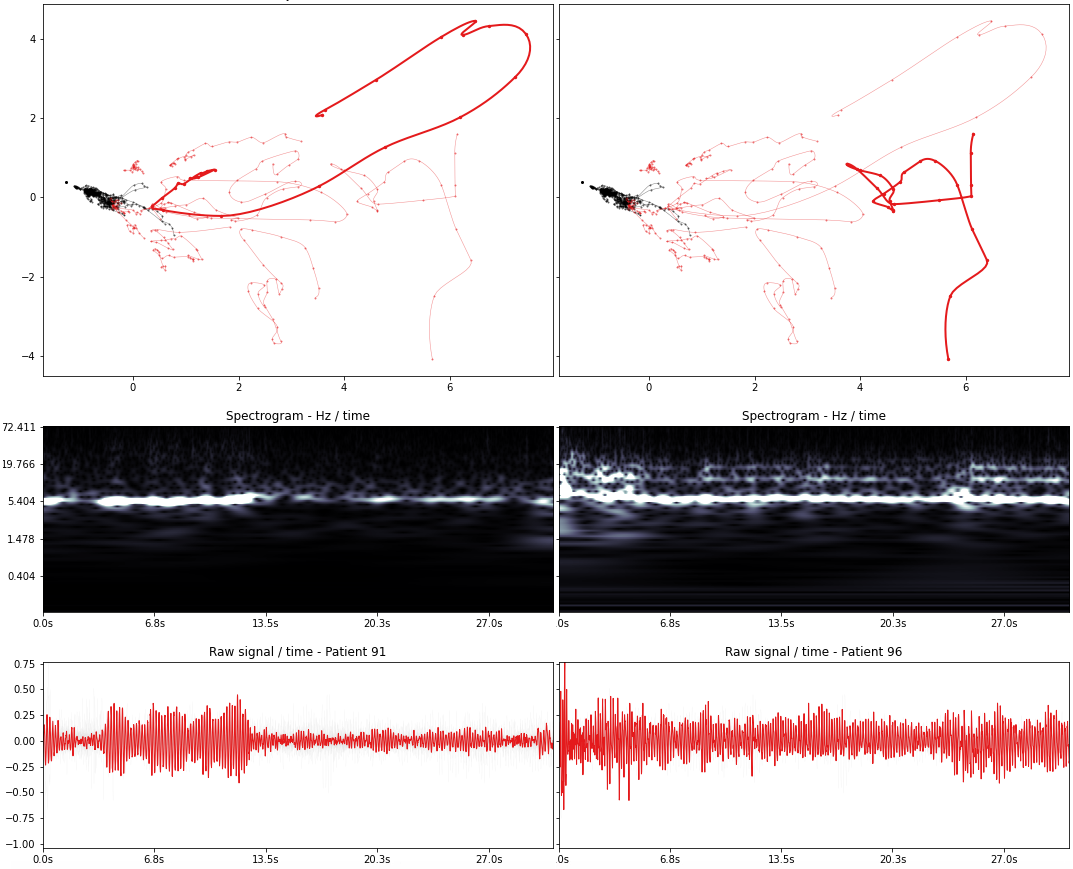
\includegraphics[width=\linewidth]{figures/nemo/exp1-9196.png}
\caption{Our tool allows selection and inspection of patients. Other than the plots shown in the figure, the tool also displays a video recording of the experiment.}
\label{fig:exp1-9196}
\end{figure*}

The projection also allows us to investigate the border between the two classes, potentially revealing subjects of interest with complex diagnoses.
\cref{fig:exp1-3942} shows two subjects whose trails are in the border and overlap each other. However, patient 39 (left) is classified as healthy, while patient 42 (right) was diagnosed with essential tremor. Comparing their signals, we see that subject 39's signal has a larger amplitude and a sharper spectrum, which to the untrained eye, it could mean that he/she suffers from tremors. However, the subject's tremors have a very high-frequency main component (over 10 Hz), which puts him/her outside the normal range for essential tremors (5--8 Hz) -- maybe the subject just drank too much coffee in the morning. His/her tremor also does not seem to be a very significant impact on other tasks. Patient 42, however, does not display obvious tremor symptoms in this particular static task, but given its classification, we must explore the reasons for the diagnosis.
Further exploration tells us that this particular patient has one side of the body more affected than the other. The condition appears to be more noticeable when performing active tasks (instead of holding static positions), as witnessed by the so-called Archimedes Spiral tests\footnote{In this drawing task, the subject is shown an Archimedean spiral, and asked to reproduced it as faithfully as possible \citep{bain}.} (\cref{fig:spirals}). Patient 42 shows tremor signals for both hands, but the tremor is much more apparent on the left.

\begin{figure*}[ht]
\centering
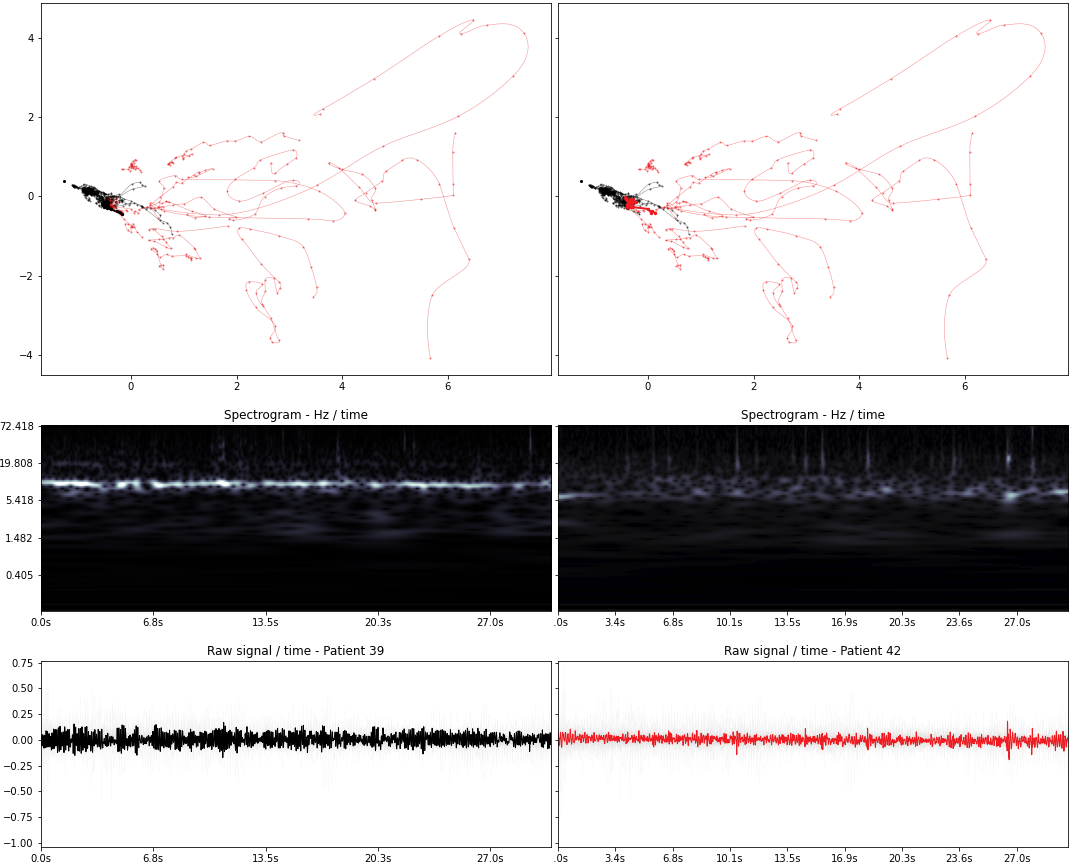
\includegraphics[width=\linewidth]{figures/nemo/exp1-3942.png}
\caption{The trail representing the patient on the right is very close to the healthy group. If we look at only his right hand during the recording of this specific task, it is hard to tell that he/she suffers from tremors, and it raises the question as to why was he/she diagnosed with tremors. Does it have a postural/unilateral aspect that is not captured in this task?
%ALEX: I think it is fine as it is.
%\eduardo{hard to see, not sure how I can make it better.}
}
\label{fig:exp1-3942}
\end{figure*}

\begin{figure*}[ht]
\centering
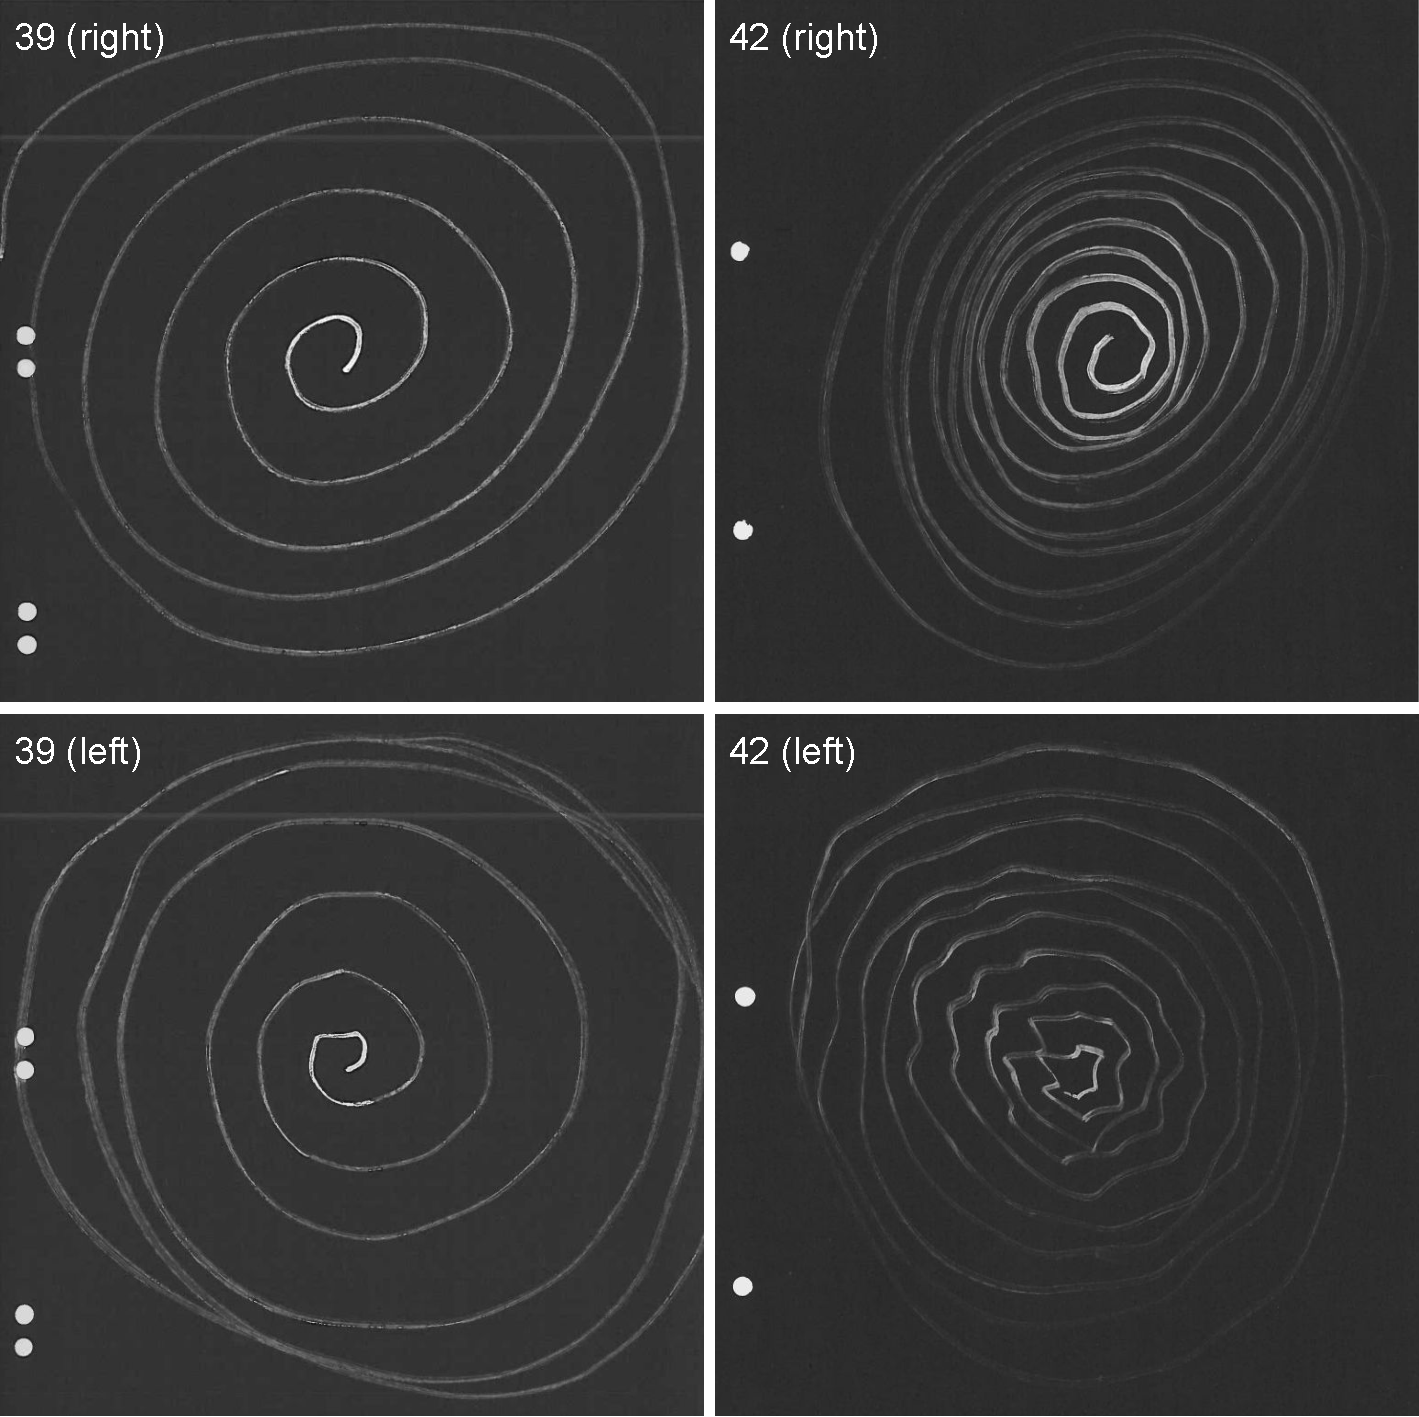
\includegraphics[width=.7\linewidth]{figures/nemo/4-spirals.pdf}
\caption{Archimedes spirals for both hands of patients 39 and 42.}
\label{fig:spirals}
\end{figure*}
    
Finally, we can notice some healthy trails reaching out into ``tremor territory'', revealing interesting subjects for investigation. One trail that attracts attention in the projection is the one of patient 3 (\cref{fig:exp1-337}-left). While most of the trail is located near other healthy patients, a part of the trail extends to the right. Looking at the spectrogram and raw signal, we can see that the patient trembles for a short period. However, the video (again, not shown here for privacy concerns) shows that this happens as the patient talks to the researchers and slightly moves his/her legs, which does not indicate an incorrect diagnosis.
Such a trail could also mean that a true essential tremor patient lost control of the suppression of the involuntary movement. The moment this happens is clearly pointed out in the projection and could have been easily not noticed in a clinical setting. We see a similar trend for patient 37 (\cref{fig:exp1-337}-right), but in this case, the movement is due to a late stop of the recording -- the sensors and camera keep going as the subject is told to return to a rest position. These recordings also help us confirm an earlier suspicion about the meaning of the northeast and southeast portions of the projection space. These are related to the ``sharpness'' of the spectrum: signals where the frequency band of 5--8 Hz tends to form the majority of the spectrum energy tend to go north-east, these ``well-behaved/well-defined'' tremors. At the same time, the direction towards the southeast of the projection is representative of more uniform spectral distributions, related to more chaotic movements.

\begin{figure*}[ht]
\centering
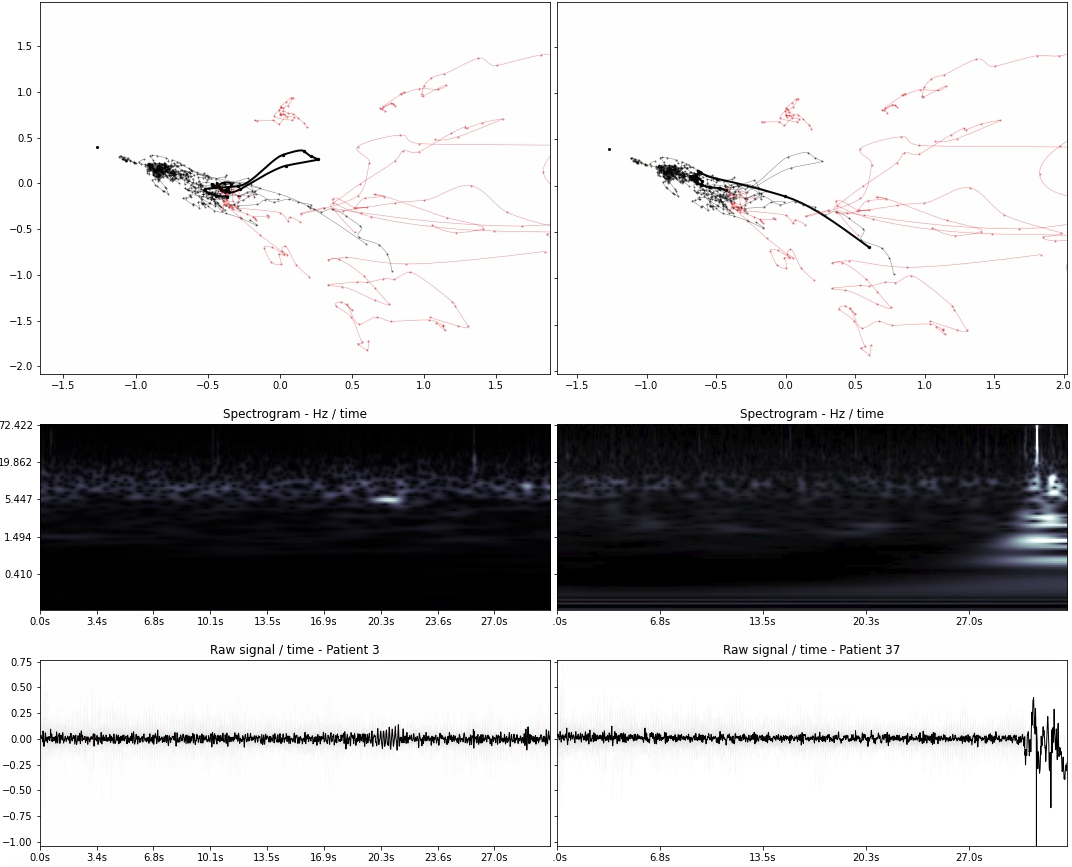
\includegraphics[width=\linewidth]{figures/nemo/exp1-337.png}
\caption{Temporary tremors on the left, and premature end of experiment on the right.}
\label{fig:exp1-337}
\end{figure*}

All the previous analysis was done atop of a single G-PCA projection. However, the other projection techniques implemented into the tool can offer different perspectives on the data, which could be useful in other tasks. \cref{fig:diff-projs} shows the results of six projection techniques for the same data. These projections show a PCD-tSNE characteristic previously discussed (\cref{sec:lambda}), namely its ability to mix characteristics of PCA (focus on distance preservation) and of tSNE (focus on neighborhood preservation) based on the setting of its $\lambda$ parameter.

\begin{figure}
\begin{tabular}{cc}
\subfloat[G-PCA]{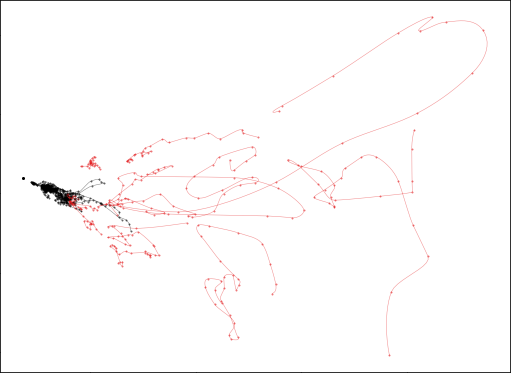
\includegraphics[width=.5\linewidth]{figures/nemo/exp1-5s-window.png}} &
\subfloat[PCD-tSNE $\lambda=.1$]{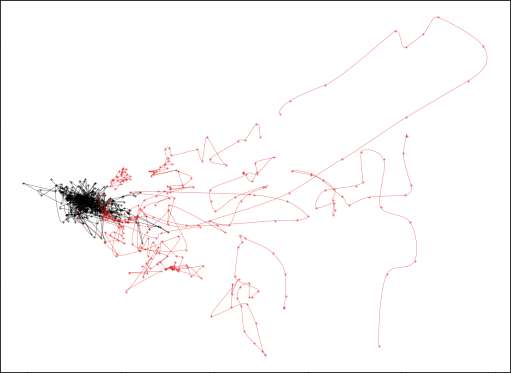
\includegraphics[width=.5\linewidth]{figures/nemo/exp1-pcd0,1.png}} \\
\subfloat[PCD-tSNE $\lambda=.001$]{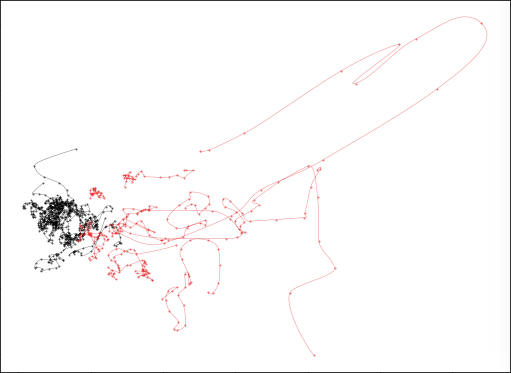
\includegraphics[width=.5\linewidth]{figures/nemo/exp1-pcd0,001.png}} &
\subfloat[PCD-tSNE $\lambda=.0001$]{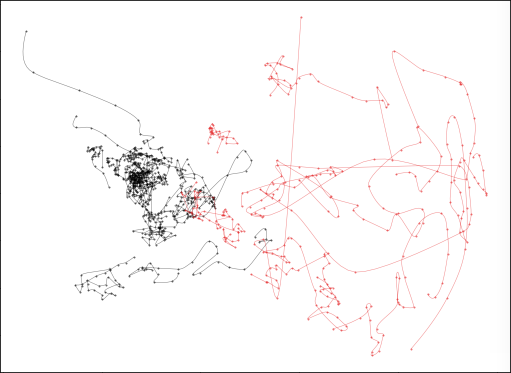
\includegraphics[width=.5\linewidth]{figures/nemo/exp1-pcd0,0001.png}}\\
\subfloat[PCD-tSNE $\lambda=.000001$]{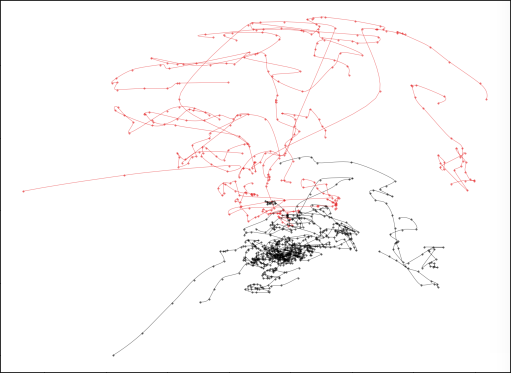
\includegraphics[width=.5\linewidth]{figures/nemo/exp1-pcd0,000001.png}} &
\subfloat[G-tSNE]{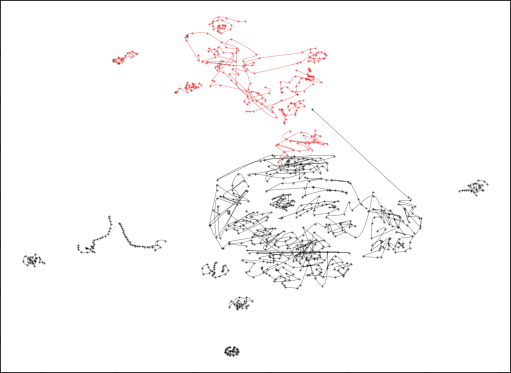
\includegraphics[width=.5\linewidth]{figures/nemo/exp1-gtsne.png}}
\end{tabular}
\caption{Different projection of the same data showing how PCD-tSNE is able to create a hybrid focus on distance preservation or neighborhood preservation depending on the $\lambda$ parameter setting.}
\label{fig:diff-projs}
\end{figure}

Our analysis so far focused on comparing control subjects to tremor patients. Another important clinical question concerns comparing different disorders and patient groups to comprehend better disorder manifestation and support challenging phenotypic classification. As previously pointed out, cross-analysis is an understudied topic supported by our tool. \cref{fig:MvsT} shows patients classified with Myoclonus and Essential Tremors on the same projection, referring to a relevant clinical question, given that Myoclonus can manifest itself in the form of periodic jerks that closely resemble tremors. Being able to perform the phenotypic classification correctly is critical for effective treatment of the disorders.
In the projections of this data, we can see some separation in the two classes. This is valuable evidence for the value of our projection-based approach, supporting our claim that it can lead to further developments in classification development.


\begin{figure}
\centering
\begin{tabular}{c}
\subfloat[G-PCA]{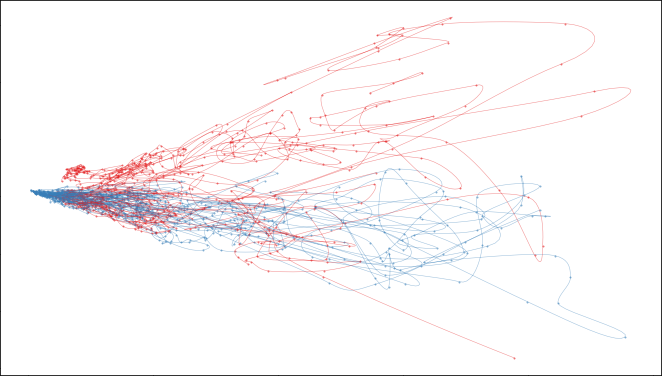
\includegraphics[width=.8\linewidth]{figures/nemo/MvsT-pca.png}} \\
\subfloat[G-tSNE]{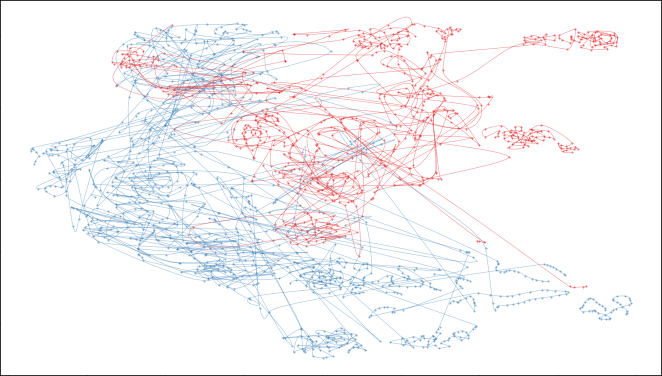
\includegraphics[width=.8\linewidth]{figures/nemo/MvsT-tsne.png}}
\end{tabular}
\caption{G-PCA and G-tSNE projections of 16 Myoclonus patients (blue) and 11 essential tremor (red) patients for the same task and sensor placement with window size of 1s and stride of 0.5s. Some separation can be seen, which is a good indicative that the methods we developed can be used to support the classification of patients groups, which is one of the ultimate goals of the NEMO project, but falls outside the scope of this thesis.}
\label{fig:MvsT}
\end{figure}


\section{Discussion}
\label{sec:nemo_discussion}
%
Given the novelty of our approach and the initial positive results obtained, several points can be discussed to improve our visual analytics tool to make it more effective for tackling phenotypic classification and exploration of EMG and accelerometer data. Below we discuss several such points and indicate directions for future work and further exploration.

\begin{itemize}
  \item \emph{What sort of insights can we get about undiagnosed patients?}
\end{itemize}
%
One possible use of our tool, which has not been properly investigated yet, is its capability as a visual \emph{classification} tool. In practice, this could be done by adding a new undiagnosed study subject to a projection such as the one in \cref{fig:MvsT}. Given the data transformations performed to construct the lower dimensional (embedding) space and/or the similarity of the subject's data compared to the other diagnosed recordings, by comparing the shape and position of the new trail to the ones already present in the projection, we can find evidence that may lead to a diagnosis (classification). Given the large number of experiments each patient performs, by using multiple projections and comparison groups, we could also draw conclusions about the circumstantial and individual aspects of the excessive and involuntary movements.

\begin{itemize}
  \item \emph{Can we identify data features that explain why patients or patient groups differ from each other in the projections?}
\end{itemize}
We addressed this goal by designing a tool that explores the data ``both ways''. In the ``forward direction'', we can take the raw data and, via many transformations and augmentation steps, create a high-level complex representation using projection trails that allow us to reason about the underlying temporal and high-dimensional structure of the dataset. The ``reverse direction'' implies taking this complex visual representation, and via interaction and group inspection, explore the features on the original data that cause the high-level representation to present specific visual features.
The analysis performed on \cref{fig:exp1-gpca,fig:exp1-9196} is a prime example of such feature identification, as the exploration we performed quickly gave us insight into the intensity (given the distance of trails to the control group) and regularity (based on the orientation of trails) of tremors.


\begin{itemize}
  \item \emph{Can we use the tool to identify which task and sensor combinations are relevant to a given diagnosis?}
\end{itemize}
Due to the size and goals of the NEMO project, we were able to collect large amounts of data from patients, asking them to perform many motion tasks, while connected to a range of state-of-the-art sensors. This is, of course, taxing on the subjects. With that in mind, and knowing that most clinical settings are not as well equipped or prepared to run such tests, one of the clinical goals of this project is to define what are (if any) the \emph{minimal} resources and methods needed to perform a confident data-driven diagnosis. This means finding combinations of sensors, tasks, comparison groups, and (pre)processing steps, that are the most suitable in support of clinical tasks. 

By creating an interactive tool in which the user can adjust all these settings and parameters on the fly, while receiving visual feedback in the form of projection trails and secondary views of the data, we give the user new ways of reasoning and interacting with the data. We also believe that the separation and visual features seen in the projections are meaningful and relate to clinical features. For example, if a combination of sensors, tasks, and user groups seem to produce good class separation in the projection, we can expect a black-box classifier to perform well in this data \citep{rauber_aid} and we expect experts to also agree with the overall structure of the data.


\begin{itemize}
  \item \emph{Can we use the tool to make data quality judgements?}
\end{itemize}
Indeed, as shown in \cref{fig:exp1-337}, we performed an analysis on subjects that were visually found out to deviate from the healthy group, in which we found that the duration of the experiment for subject 37 deviated from the duration of the recording. In the same figure, we see a small black dot to the left of the control group that indicates the recording of a patient for which this particular sensor was not correctly attached. 

\begin{itemize}
  \item \emph{How should we continue development of this tool?}
\end{itemize}
There are many promising directions for future development that address current limitations in our tool: For example, all our current analyses are now done based on \emph{one} selected task and \emph{one} sensor at a time. We believe that it would be advantageous to perform a unified analysis on multiple sensors and tasks. This could lead to a better understanding of postural/circumstantial (depending on the task or patient focus) and individual (unilateral or only certain limbs affected) appearance of certain involuntary movements.

Additionally, in its current state, our tool performs well only for static tasks, i.e., tasks in which patients are expected to hold a position for a specific amount of time. However, many dynamic tasks are of great relevance for specific diagnoses, but due to the complexity of the signal, we are unable to extract relevant information for motion disorder analysis. Correctly handling this data would imply the development of a series of additional preprocessing steps that fall outside this thesis's scope.

Given the goals of the NEMO project, it is important to face the problems of visual analytics and classification as one. This chapter focuses on the former, but there are works in the literature that present combined approaches \citep{Graving2020.07.17.207993,rauber_aid} which could be of benefit to the clinical tasks we want to improve. 

Lastly, we focus only on EMG, accelerometer, and 2D video data. It could be beneficial to add support to exploring the extra data modalities extracted during the experiments.

% \eduardo{Jelle suggestions: \\
%     Can we add individuals to the projection and get an idea to which patient group they belong? \\
%     Can we identify data features that explain why patient groups differ from each other in the projects? \\
%     Does this solve specific issues experienced using current methodology? \\
%     How should we continue development of this tool? \\
%     What are the limitations of this tool? \\
%     Are we able to find nuances within patient groups (interindividual differences)? \\
%     Can we also use the tool to make data quality judgements? \\
%     No single useful projection method. Combination of views is best. \\
%     Use reverse projections (PCA and even the NN based one from Alex) to learn about the feature space.
% }

\section{Conclusions}

We presented a real-world application of our new dynamic projection methods in the context of hyperkinetic movement disorder analysis. We show evidence of the usefulness of these methods in support of motion data analysis.

We introduced the problem, described how we transform the data collected during clinical experiments, proposed a visual analytics tool designed to support the exploration of this complex dataset, and showed examples of data explorations that led to valuable clinical insights.

This is a preliminary investigation, and many points are still open, e.g., the actual construction of an automatic classifier based on such data, questions regarding the clinical usage of dynamic projections, the design of sophisticated UIs for medical professionals, among other directions of future work. Nevertheless, our work showed that projections have the potential to be useful in exploring temporal multidimensional data coming from a complex real-world problem.